%PROJETO

\chapter{ALGORITMO DE LEITURA DA REDE DE PETRI}

Neste cap\'itulo ser\'a apresentado o algoritmo de leitura da rede de petri, o algoritmo de aplica\c{c}\~ao do TCS e a interface gr\'afica.

\section{Algoritmo de leitura da Rede de Petri}

O algoritmo de leitura e a aplica\c{c}\~ao do TCS seguem os seguintes passos.
 \begin{itemize}
 	\item Passo 1: Modelagem do sistema em Redes de Petri;
 	\item Passo 2: Inser\c{c}\~ao da modelagem na ferramenta;
 	\item Passo 3: Adi\c{c}\~ao de equa\c{c}\~oes de restri\c{c}\~ao;
 	\item Passo 4: Extra\c{c}\~ao da RdP com o supervis\'orio;
 	\item Passo 5: Avalia\c{c}\~ao das propriedades da RdP na ferramenta de modelagem;
 	\item Passo 6: Execu\c{c}\~ao do conversor para c\'odigo implementa\'el;
 	\item Passo 7: Implementa\c{c}\~ao do c\'odigo em um controlador.
 \end{itemize}


\section{Modelagem do sistema em Redes de Petri}
O usu\'ario dever\'a modelar a planta em uma ferramenta que permita a exporta\c{c}\~ao do modelo em formato PNML (Petri Net Markup Language). Esse formato \'e regido pela ISO/IEC 15909-3, e utiliza como base a linguagem de marca\c{c}\~ao XML (eXtensible Markup Language) afim de padronizar um formato de arquivo para a RdP \cite{pnmlorg}. No ap\^endice ?? \'e apresentado a estrutura b\'asica de um arquivo PNML.

\section{Interface gr\'afica}
A interface gr\'afica tem por objetivo facilitar as entradas de dados pelo usu\'ario. Nela o usu\'ario indica o arquivo PNML, adiciona as especifica\c{c}\~oes da planta e gera os arquivos da nova RdP e o c\'odigo implement\'avel. 

Na figura~\ref{fig:interfacegrafica} \'e apresentado a interface gr\'afica.

\begin{figure}[!htb]
	%\captionsetup{width=0.97\textwidth}
	\caption[Interface gr\'afica do projeto PN2IC.]{Interface gr\'afica do projeto PN2IC.}
	\label{fig:interfacegrafica}
	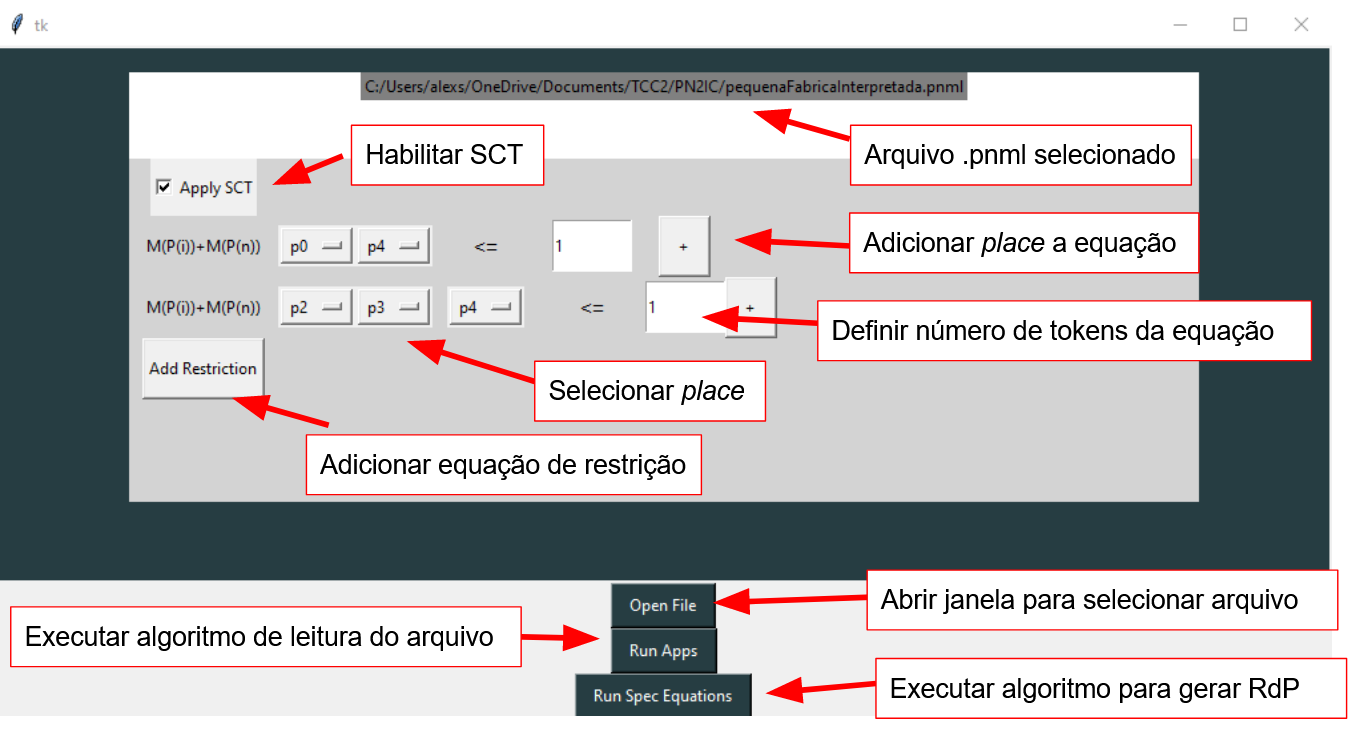
\includegraphics[width=16cm]{./figuras/INTERFACE_GRAFICA_PN2IC.png}\centering
	\fonte{Autoria pr\'opria.}
\end{figure}

\section{Extra\c{c}\~ao das informa\c{c}\~oes da RdP}
Ap\'os a escolha do arquivo PNML pelo usu\'ario, a ferramenta executa uma extra\c{c}\~ao de informa\c{c}\~oes da RdP e armazena de forma orientada a objetos. Para isso, foi criado tr\^es classes; Place, Transition e Arc. Cada classe de objeto representa um elemento da rede, Place representa o Lugar e tem como propriedade seu c\'odigo identidade, nome, r\'otulo e se h\'a marca\c{c}\~ao inicial. Transition tamb\'em possui propriedades como identidade, nome e r\'otulo.
O caso mais especial \'e da classe Arc, que \'e o arco que interliga os elementos de uma RdP. Arc possui como propriedades a sua identidade, a fonte de onde parte o arco e o seu alvo onde termina o arco. Tamb\'em possui m\'etodos de classe que retornam uma lista de transi\c{c}\~oes dado uma identidade de um Lugar, s\~ao duas fun\c{c}\~oes que retornam transi\c{c}\~oes que precedem ou sucedem dado Lugar. As propriedades das classes s\~ao ilustradas na figura~\ref{fig:classes}.

\begin{figure}[!htb]
	%\captionsetup{width=0.97\textwidth}
	\caption[Classes de objetos participantes da RdP.]{Classes de objetos participantes da RdP.}
	\label{fig:classes}
	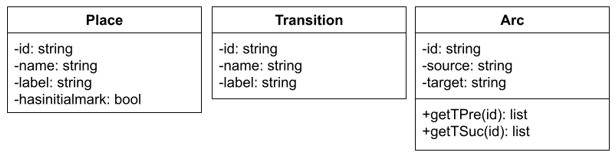
\includegraphics[width=16cm]{./figuras/CLASSES.png}\centering
	\fonte{Autoria pr\'opria.}
\end{figure}

\section{Abordagem h\'ibrida de Uzam e Wonham}

No trabalho \cite{UzamWonham2005}, \'e apresentado uma abordagem h\'ibrida para o controle supervis\'orio de SEDs atrav\'es do acoplamento de supervis\'orios RW (Ramadge Wonham) em Redes de Petri. Este trabalho consiste em simplificar uma RdP, de um modelo n\~ao control\'avel, e representar a rede e sua especifica\c{c}\~ao, que \'e um conjunto de estados proibidos, em aut\^omatos e ent\~ao aplicar a TCS para obter o supervis\'orio RW. O supervis\'orio RW \'e respresentado em RdP passando a se chamar auto-net e este \'e acoplado no modelo inicial n\~ao control\'avel. Na ~\ref{fig:uzamcontrol} \'e apresentado a abordagem h\'ibrida de um controle supervis\'orio de uma RdP.

\begin{figure}[!htb]
	%\captionsetup{width=0.97\textwidth}
	\caption[Controle supervis\'orio de um SED baseado na abordagem de \cite{UzamWonham2005}.]{Controle supervis\'orio de um SED baseado na abordagem de \cite{UzamWonham2005}.}
	\label{fig:uzamcontrol}
	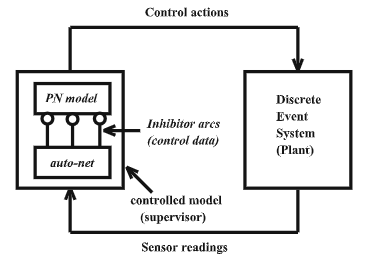
\includegraphics[width=16cm]{./figuras/UZAMCONTROL.png}\centering
	\fonte{\cite{UzamWonham2005}}
\end{figure}



\section{Abordagem aplicada no projeto}

Neste projeto, a metodologia aplicada \'e baseada na abordadem h\'ibrida de \cite{UzamWonham2005}. As diferen\c{c}as ficam por conta da n\~ao simplifica\c{c}\~ao da RdP inicial e a n\~ao utiliza\c{c}\~ao do m\'etodo supervisor\'orio RW.

Inspirado no exemplo pequena fa\'abrica de \cite{apostilacury}, na figura ~\ref{fig:pqnafab} \'e apresentado uma modelagem em RdP que representa uma pequena f\'abrica. O conjunto de lugares p0 e p1 representam uma c\'elula de usinagem, p4 um buffer (fila) e o conjunto p2 e p3 uma c\'elula de pintura. Um CLP ir\'a comandar a atua\c{c}\~ao das c\'elulas de fabrica\c{c}\~ao e para isso uma l\'ogica discreta e sequencial deve ser desenvolvida, a l\'ogica dever\'a contar com intertravamentos para garantir que, por exemplo, um operador for\c{c}e a atua\c{c}\~ao atrav\'es de comando manual. Esse intertravamento \'e o que comp\~oe o sistema de supervis\~ao.
As fichas (tokens) em p1 representam ociosidade da usinagem, j\'a em p0 representam o trabalho de usinagem. Em p4 representam pe\c{c}as em aguardo e em p3 ociosidade na pintura e p2 em trabalho de pintura.\

\begin{figure}[!htb]
	%\captionsetup{width=0.97\textwidth}
	\caption[Modelagem de uma pequena f\'abrica.]{Modelagem de uma pequena f\'abrica.}
	\label{fig:pqnafabrica}
	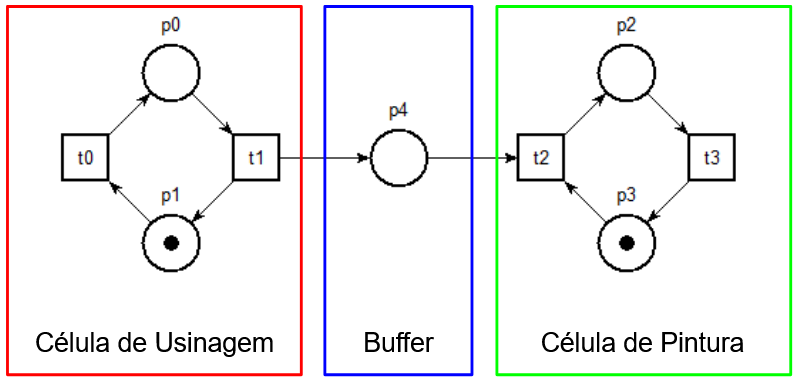
\includegraphics[width=16cm]{./figuras/PQNAFAB.png}\centering
	\fonte{Autoria pr\'opria.}
\end{figure}

A especifica\c{c}\~ao deste projeto \'e que n\~ao haja overflow (ac\'umulo de pe\c{c}as pela c\'elula de usinagem) e nem underflow (in\'icio do processo de pintura sem pe\c{c}as dispon\'iveis) no buffer. Pela pr\'opria propriedade da RdP, em permitir o disparo das transi\c{c}\~oes somente quando os lugares que precedem as transi\c{c}\~oes possuem marca\c{c}\~ao maior ou igual ao peso do arco, \'e impedido o disparo de t2 sem que haja pe\c{c}a em p4. O overflow ficar\'a por conta de um supervisor. Sendo t0 uma transi\c{c}\~ao contro\'avel e t1 um sinal de finaliza\c{c}\~ao do trabalho de usinagem, se faz necess\'ario impedir que a c\'elula de usinagem inicie seu processo quando h\'a pe\c{c}a em p4, sendo assim, a equa\c{c}\~ao da especifica\c{c}\~ao \'e M(p0) + M(p4) <= 1. A soma das fichas de p0 e p4 sempre deve ser menor ou igual a zero, com essa essa especifica\c{c}\~ao garante-se o intertravamento de t0 inibindo o overflow de p4.




